\tikzsetexternalprefix{tikz/}	% set subfolder
\tikzsetnextfilename{IRIS}
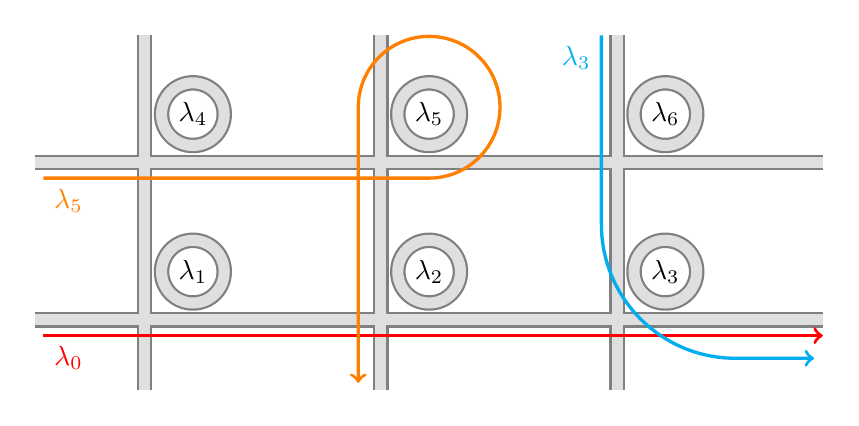
\begin{tikzpicture}[
		baseline,
		wave/.style	={ 
			very thick, line cap=butt, ->,
			%rounded corners=128pt,
		},
		guide/.style 	={ double=gray!25, double distance=4pt,
			thick, draw=black!50,
			rounded corners=4pt, line join=round, line cap=butt,
		},
		ring/.style 		={ circle, radius=64pt,
			double=gray!25, double distance=4pt,
			thick, draw=black!50,
			rounded corners=8pt, line join=round,
		},
	]
	
	\def\mylist{ 0/0/1, 3/0/2, 6/0/3, 0/2/4, 3/2/5, 6/2/6}
	
	% draw rings
	\foreach \x/\y/\n in \mylist
		\node [ring] (ring_\n) at (\x,\y) {$\lambda_\n$};
	
	% draw waveguides
	\draw [guide]
			% insert the horizontal wgs here
			(ring_1.south)++(-2,-0.2) -- ++(10,0)
			(ring_4.south)++(-2,-0.2) -- ++(10,0)
			% insert the vertical wgs here
			(ring_1.west)++(-0.2,-1.5) -- ++(0,4.5)
			(ring_2.west)++(-0.2,-1.5) -- ++(0,4.5)
			(ring_3.west)++(-0.2,-1.5) -- ++(0,4.5);
			
	% draw waves
	\draw [wave, red] (ring_1.south)++(-1.9,-0.4) node [below right] {$\lambda_0$} -- ++(9.9,0);
	\draw [wave, orange] (ring_4.south)++(-1.9,-0.4) node [below right] {$\lambda_5$} -- ++(4.9,0)
				arc (-90:180:0.9) -- ++(0,-3.5);
	\draw [wave, cyan] (ring_6.west)++(-0.4, 1) node [below left] {$\lambda_3$} -- ++(0,-2.4)
				arc (180:270:1.7) -- ++(1,0);
	
\end{tikzpicture}
